\chapter{More Results from the Fitting of the Extended Schmidt Law in M31}
\pagestyle{plain}
\label{app:es,figs}
\myappendices

Section~\ref{sec: sfl} discusses testing the extended Schmidt law and shows results for one SFR/gas tracer combination. Here we present the plots for the remaining SFR/gas tracer combinations.

\begin{figure}
    \centering
    \begin{subfigure}[b]{\textwidth}
        \centering
        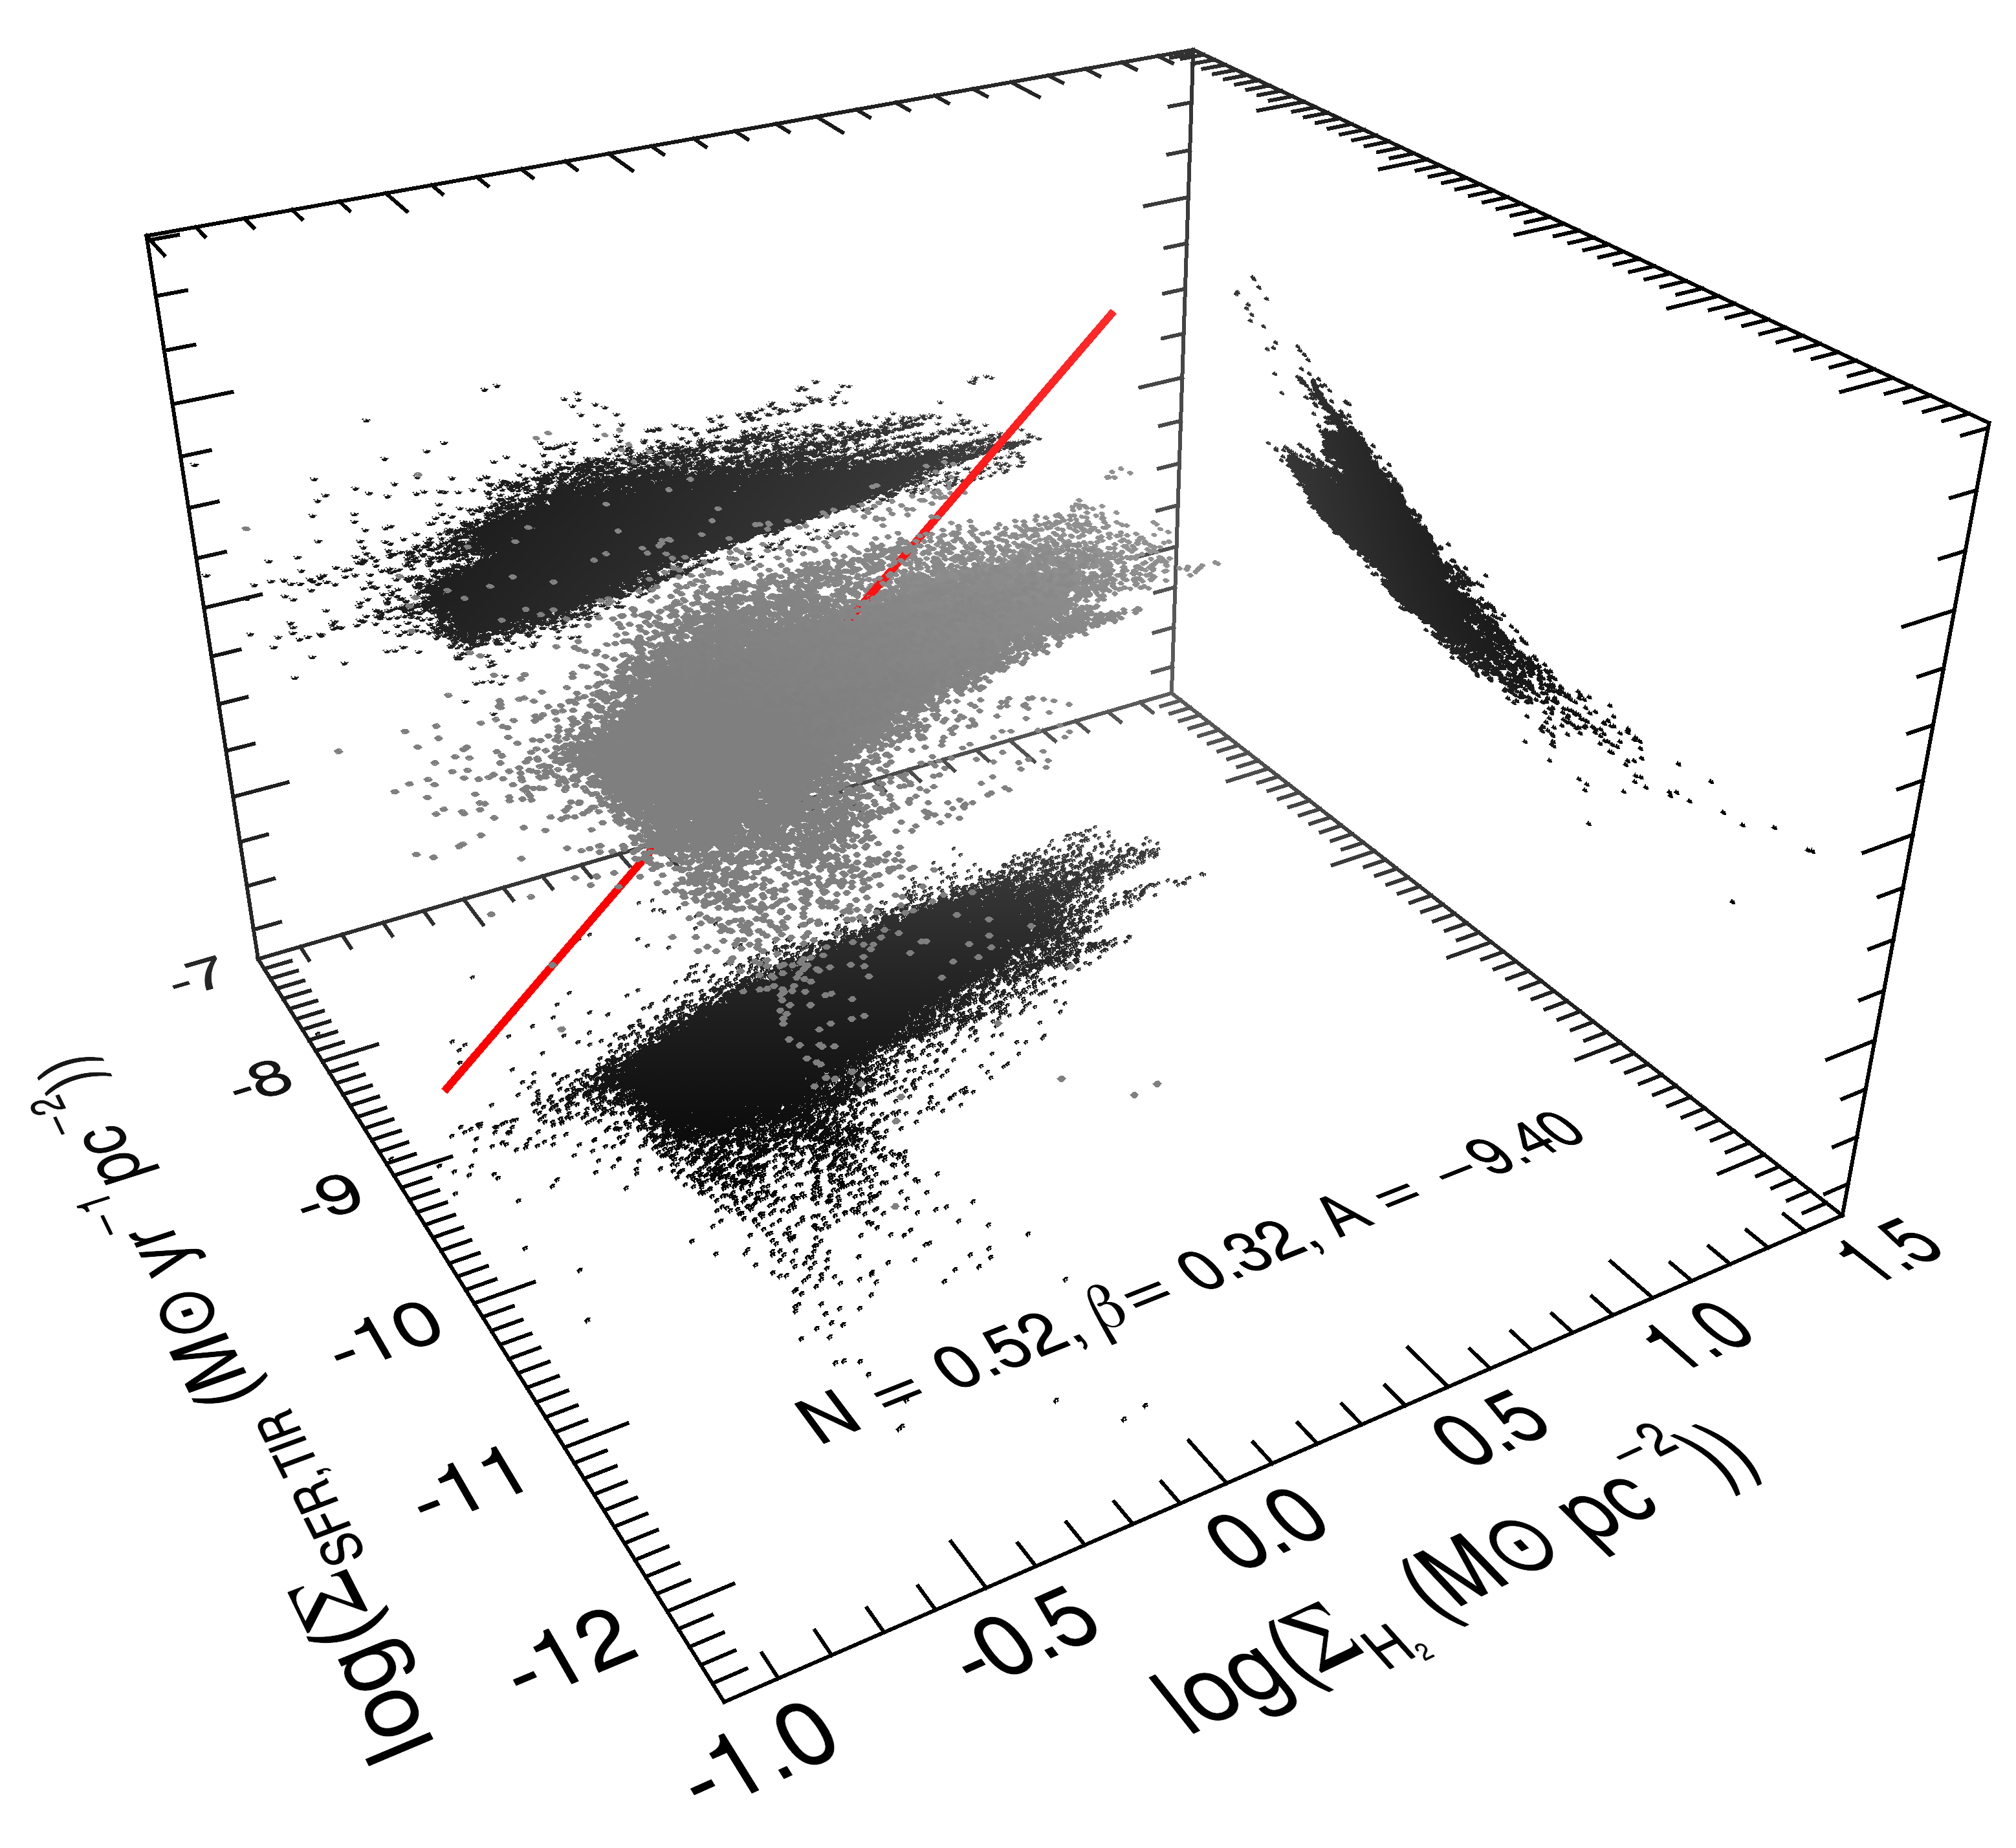
\includegraphics[width=0.5\textwidth]{../image_paper1/es_tot_fir_vs_h2.png}
        \captionsetup{font=tiny}
        \caption{Surface density of SFR(TIR) vs surface density of H$_2$ and surface density of stellar mass ($z$-axis) }
        \label{fig:es,all,fir,h2}
    \end{subfigure}
    \hfill
    \begin{subfigure}[b]{\textwidth}
        \centering
        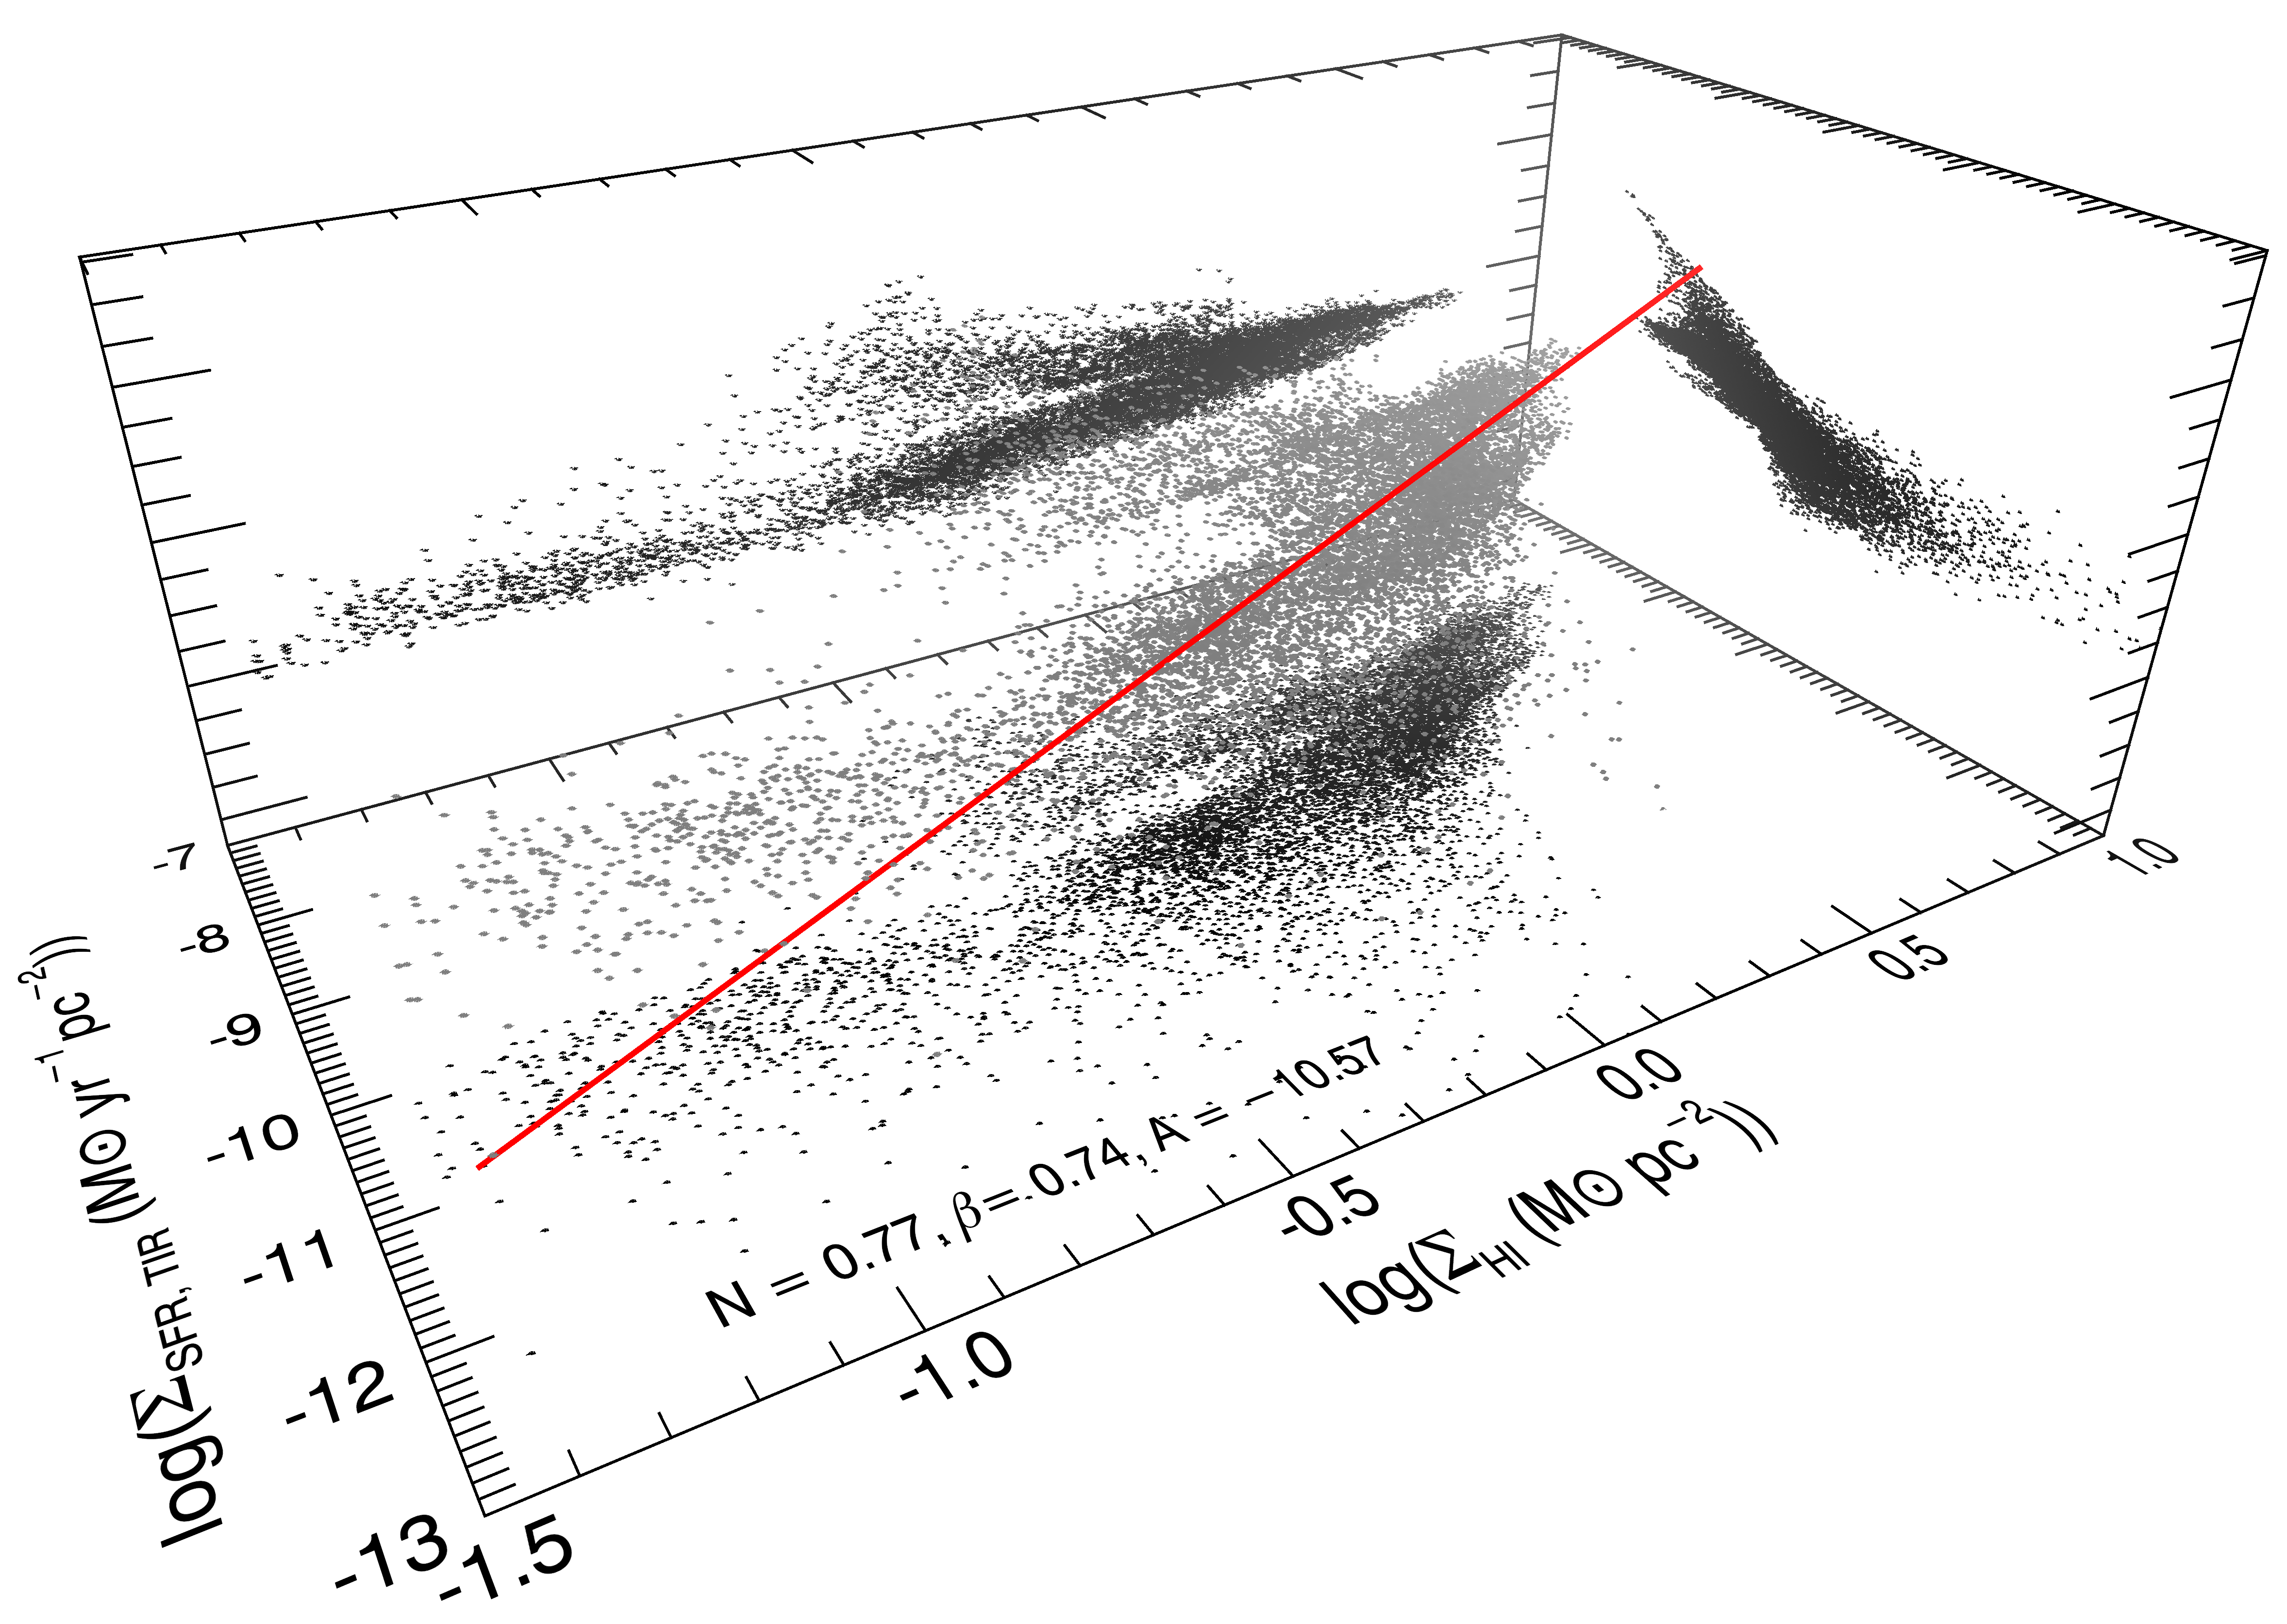
\includegraphics[width=0.5\textwidth]{../image_paper1/es_tot_fir_vs_hi2.png}
        \captionsetup{font=tiny}
        \caption{Surface density of SFR(TIR) vs surface density of \hi\ and surface density of stellar mass ($z$-axis) }
        \label{fig:es,all,fir,hi}
    \end{subfigure}
    \hfill
   \begin{subfigure}[b]{\textwidth}
        \centering
        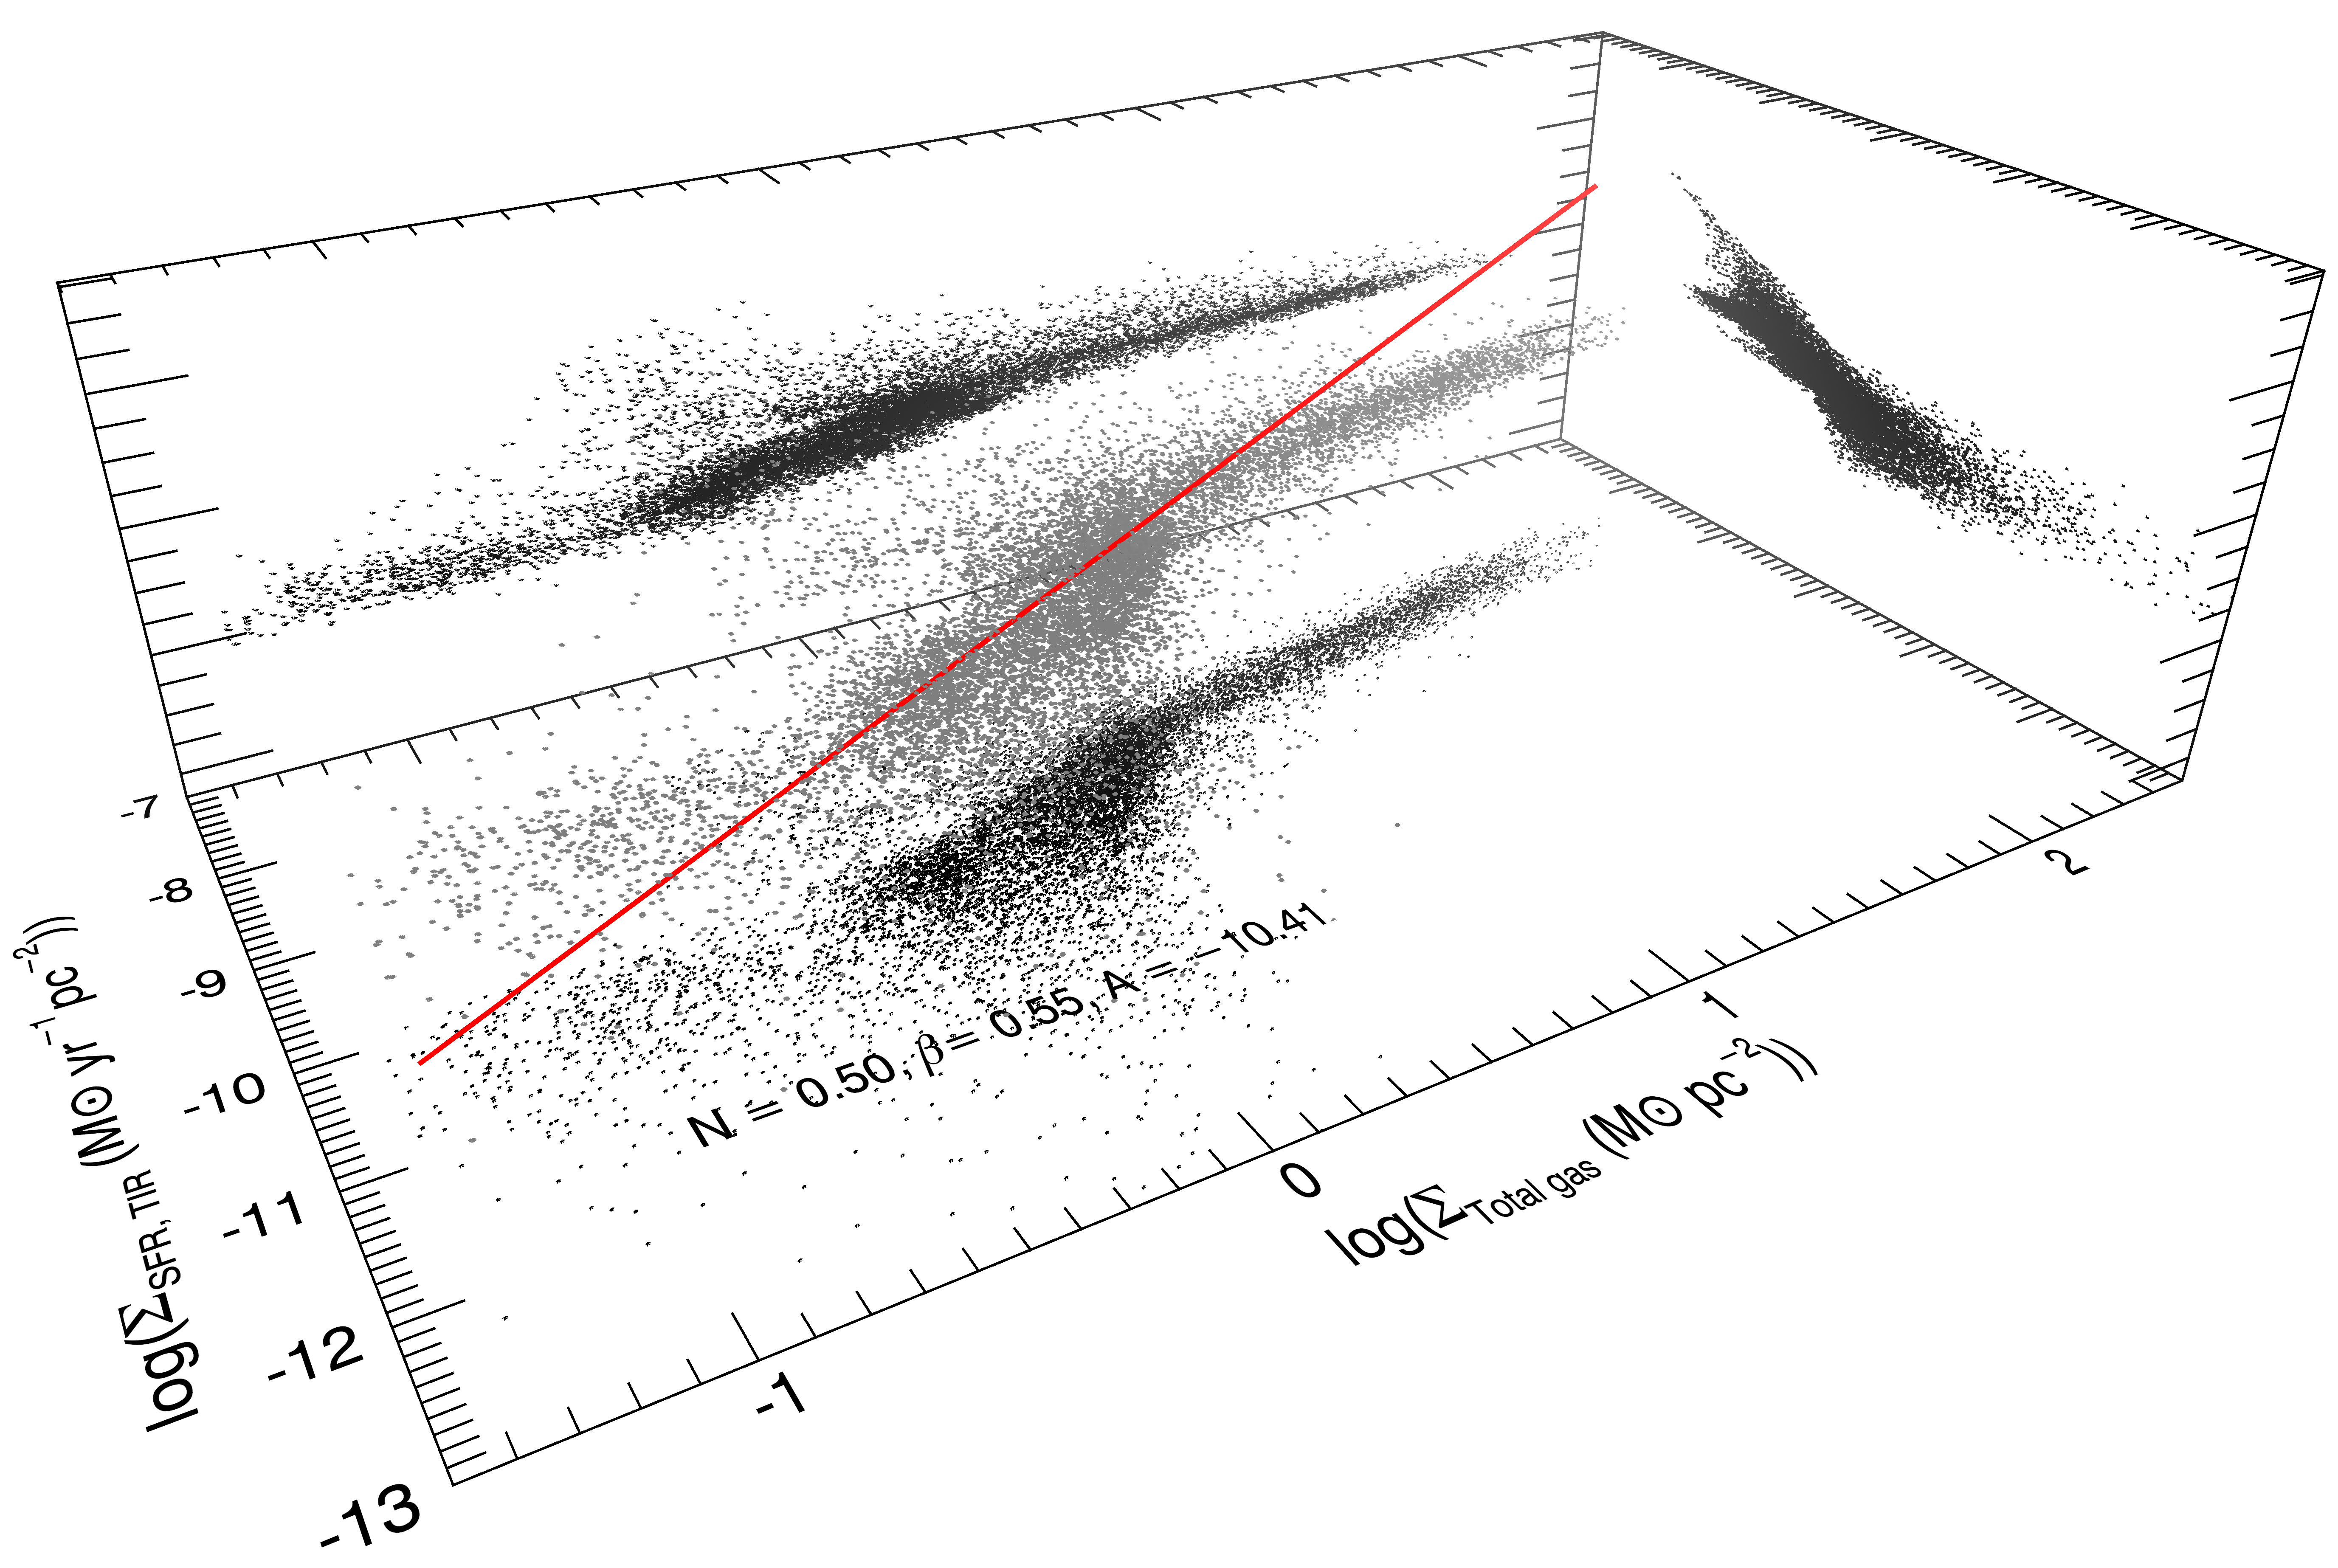
\includegraphics[width=0.5\textwidth]{../image_paper1/es_tot_fir_vs_tot2_f.png}
        \captionsetup{font=tiny}
        \caption{Surface density of SFR(TIR) vs surface density of total gas and surface density of stellar mass ($z$-axis)}
        \label{fig:es,all,fir,tot}
    \end{subfigure}
       \caption[Same as Fig.~\ref{fig:es,all,fuv,tot}, but here the surface density of the SFR(TIR) versus three gas tracer are used]{Same as Fig.~\ref{fig:es,all,fuv,tot}. Here, from top to bottom plots show the surface density of the SFR(TIR) vs. surface density of H$_2$, surface density of \hi\, and the surface density of total gas, respectively. As in Fig.~\ref{fig:ks_all}, the analyses use different pixel sizes: each point in the plots with the surface density of H$_2$ as a tracer of gas mass represents a region of size $\sim$30~pc and each point in the plots with the surface density of \hi\ or total gas mass represents a region of size $\sim$155~pc. Solid lines show the best fit, using the mean value of the ranges in Table~\ref{table:res}.}
       \label{fig:es,fir}
\end{figure}


\begin{figure}
    \centering
     \begin{subfigure}[b]{0.5\textwidth}
        \centering
        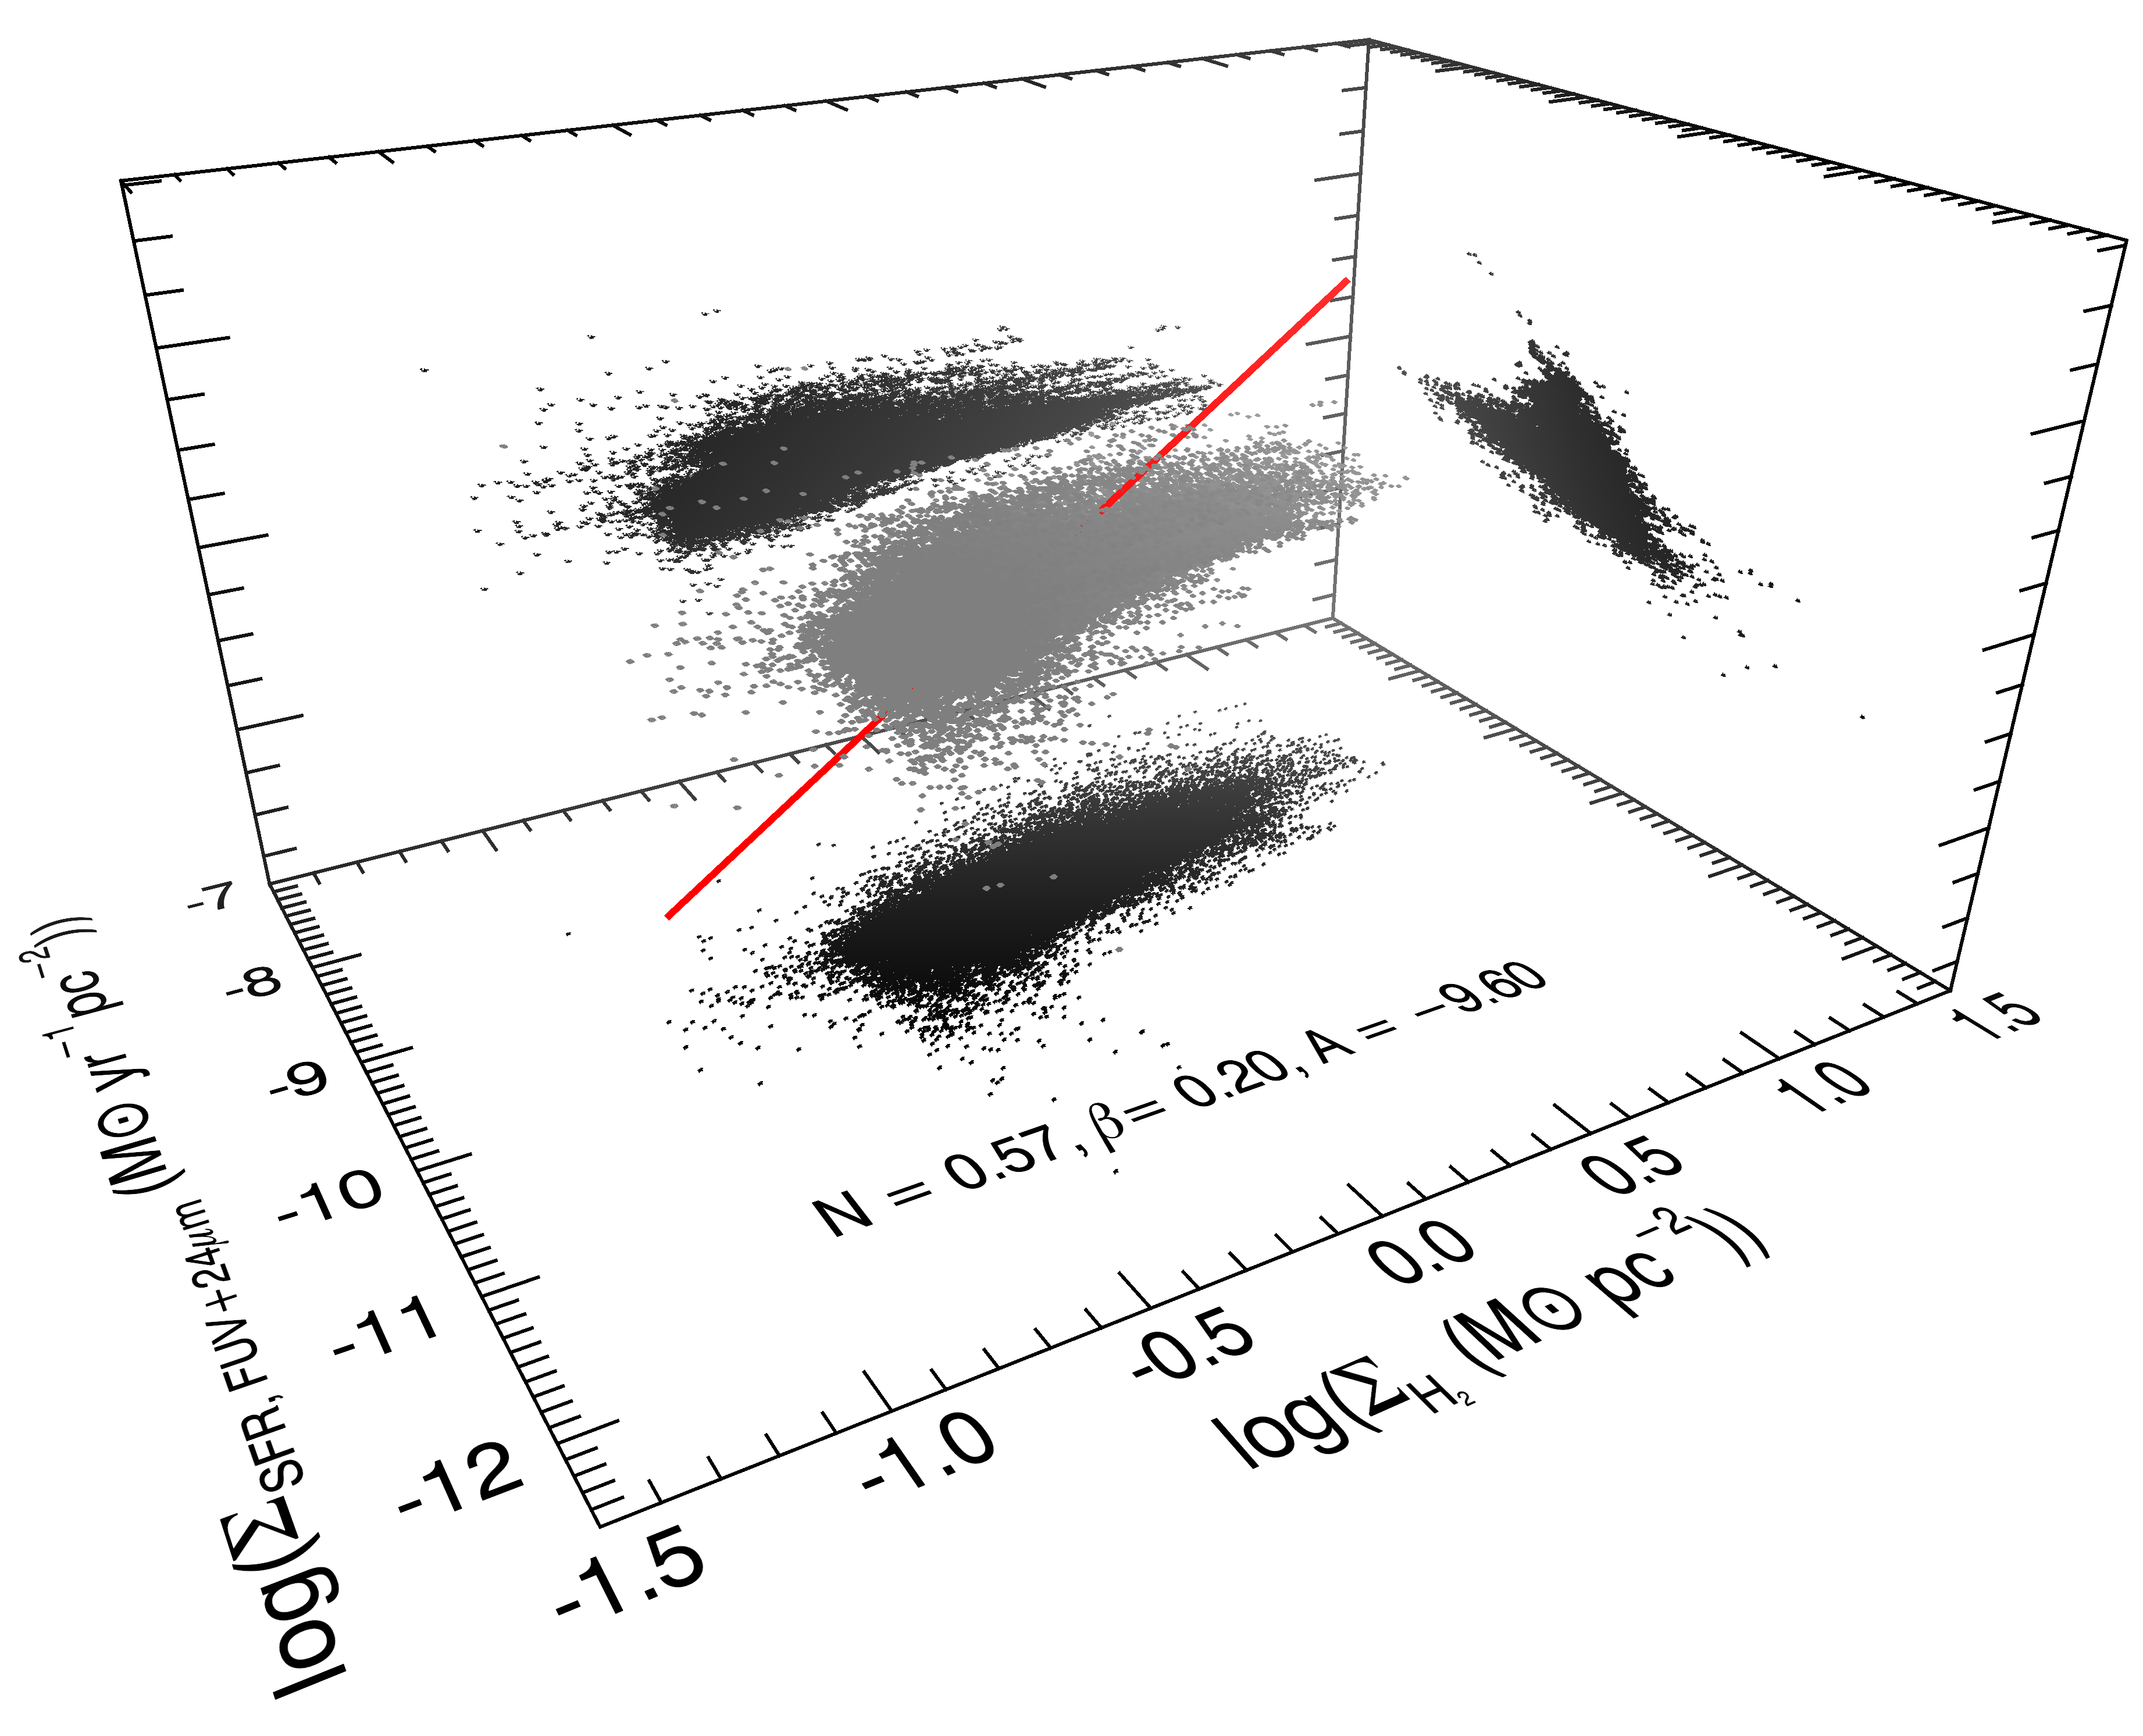
\includegraphics[width=\textwidth]{../image_paper1/es_tot_fuv_vs_h22_f.png}
        \captionsetup{font=tiny}
        \caption{Surface density of SFR(FUV+24~$\mu$m) vs surface density of H$_2$ and surface density of stellar mass ($z$-axis)}
        \label{fig:es,all,fuv,h2}
    \end{subfigure}
     \hfill
   \begin{subfigure}[b]{0.5\textwidth}
        \centering
        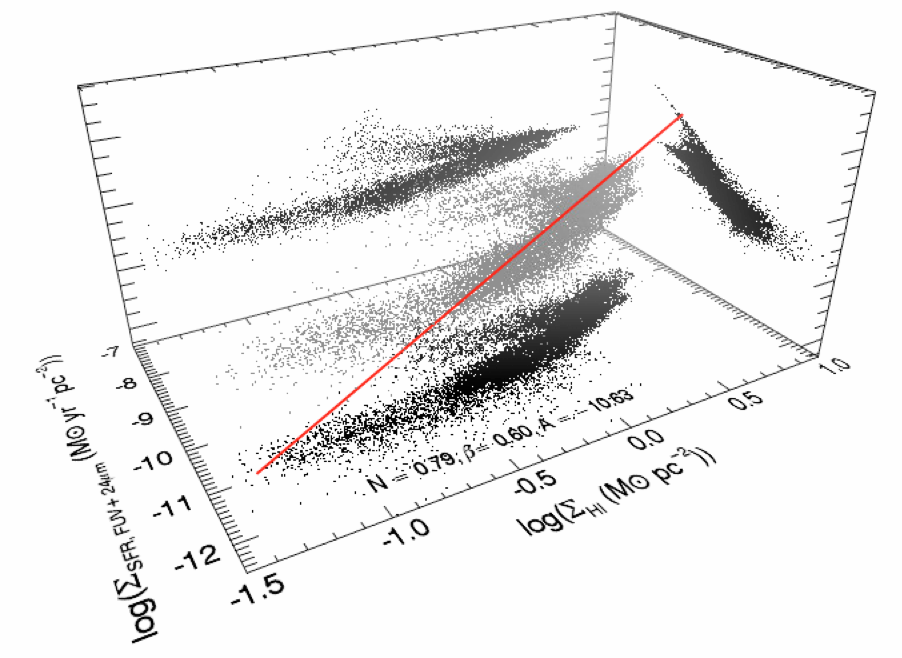
\includegraphics[width=\textwidth]{../image_paper1/es_tot_fuv_vs_hi2.png}
        \captionsetup{font=tiny}
        \caption{Surface density of SFR(FUV+24~$\mu$m) vs surface density of \hi\ and surface density of stellar mass ($z$-axis)}
        \label{fig:es,all,fuv,hi}
    \end{subfigure}
   \caption[Same as Fig.~\ref{fig:es,fir}, but in this figure we used FUV $+$ 24~$\mu$m as a tracer of the SFR]{Same as Fig.~\ref{fig:es,fir}, but in this figure we used FUV $+$ 24~$\mu$m as a tracer of the SFR. The plot of the surface density of the SFR(FUV+24~$\mu$m) vs the surface density of the total gas is shown in Fig.~\ref{fig:es,all,fuv,tot} in the main text.}
\end{figure}

         
\begin{figure}
  \centering
   \begin{subfigure}[b]{0.5\textwidth}
        \centering
        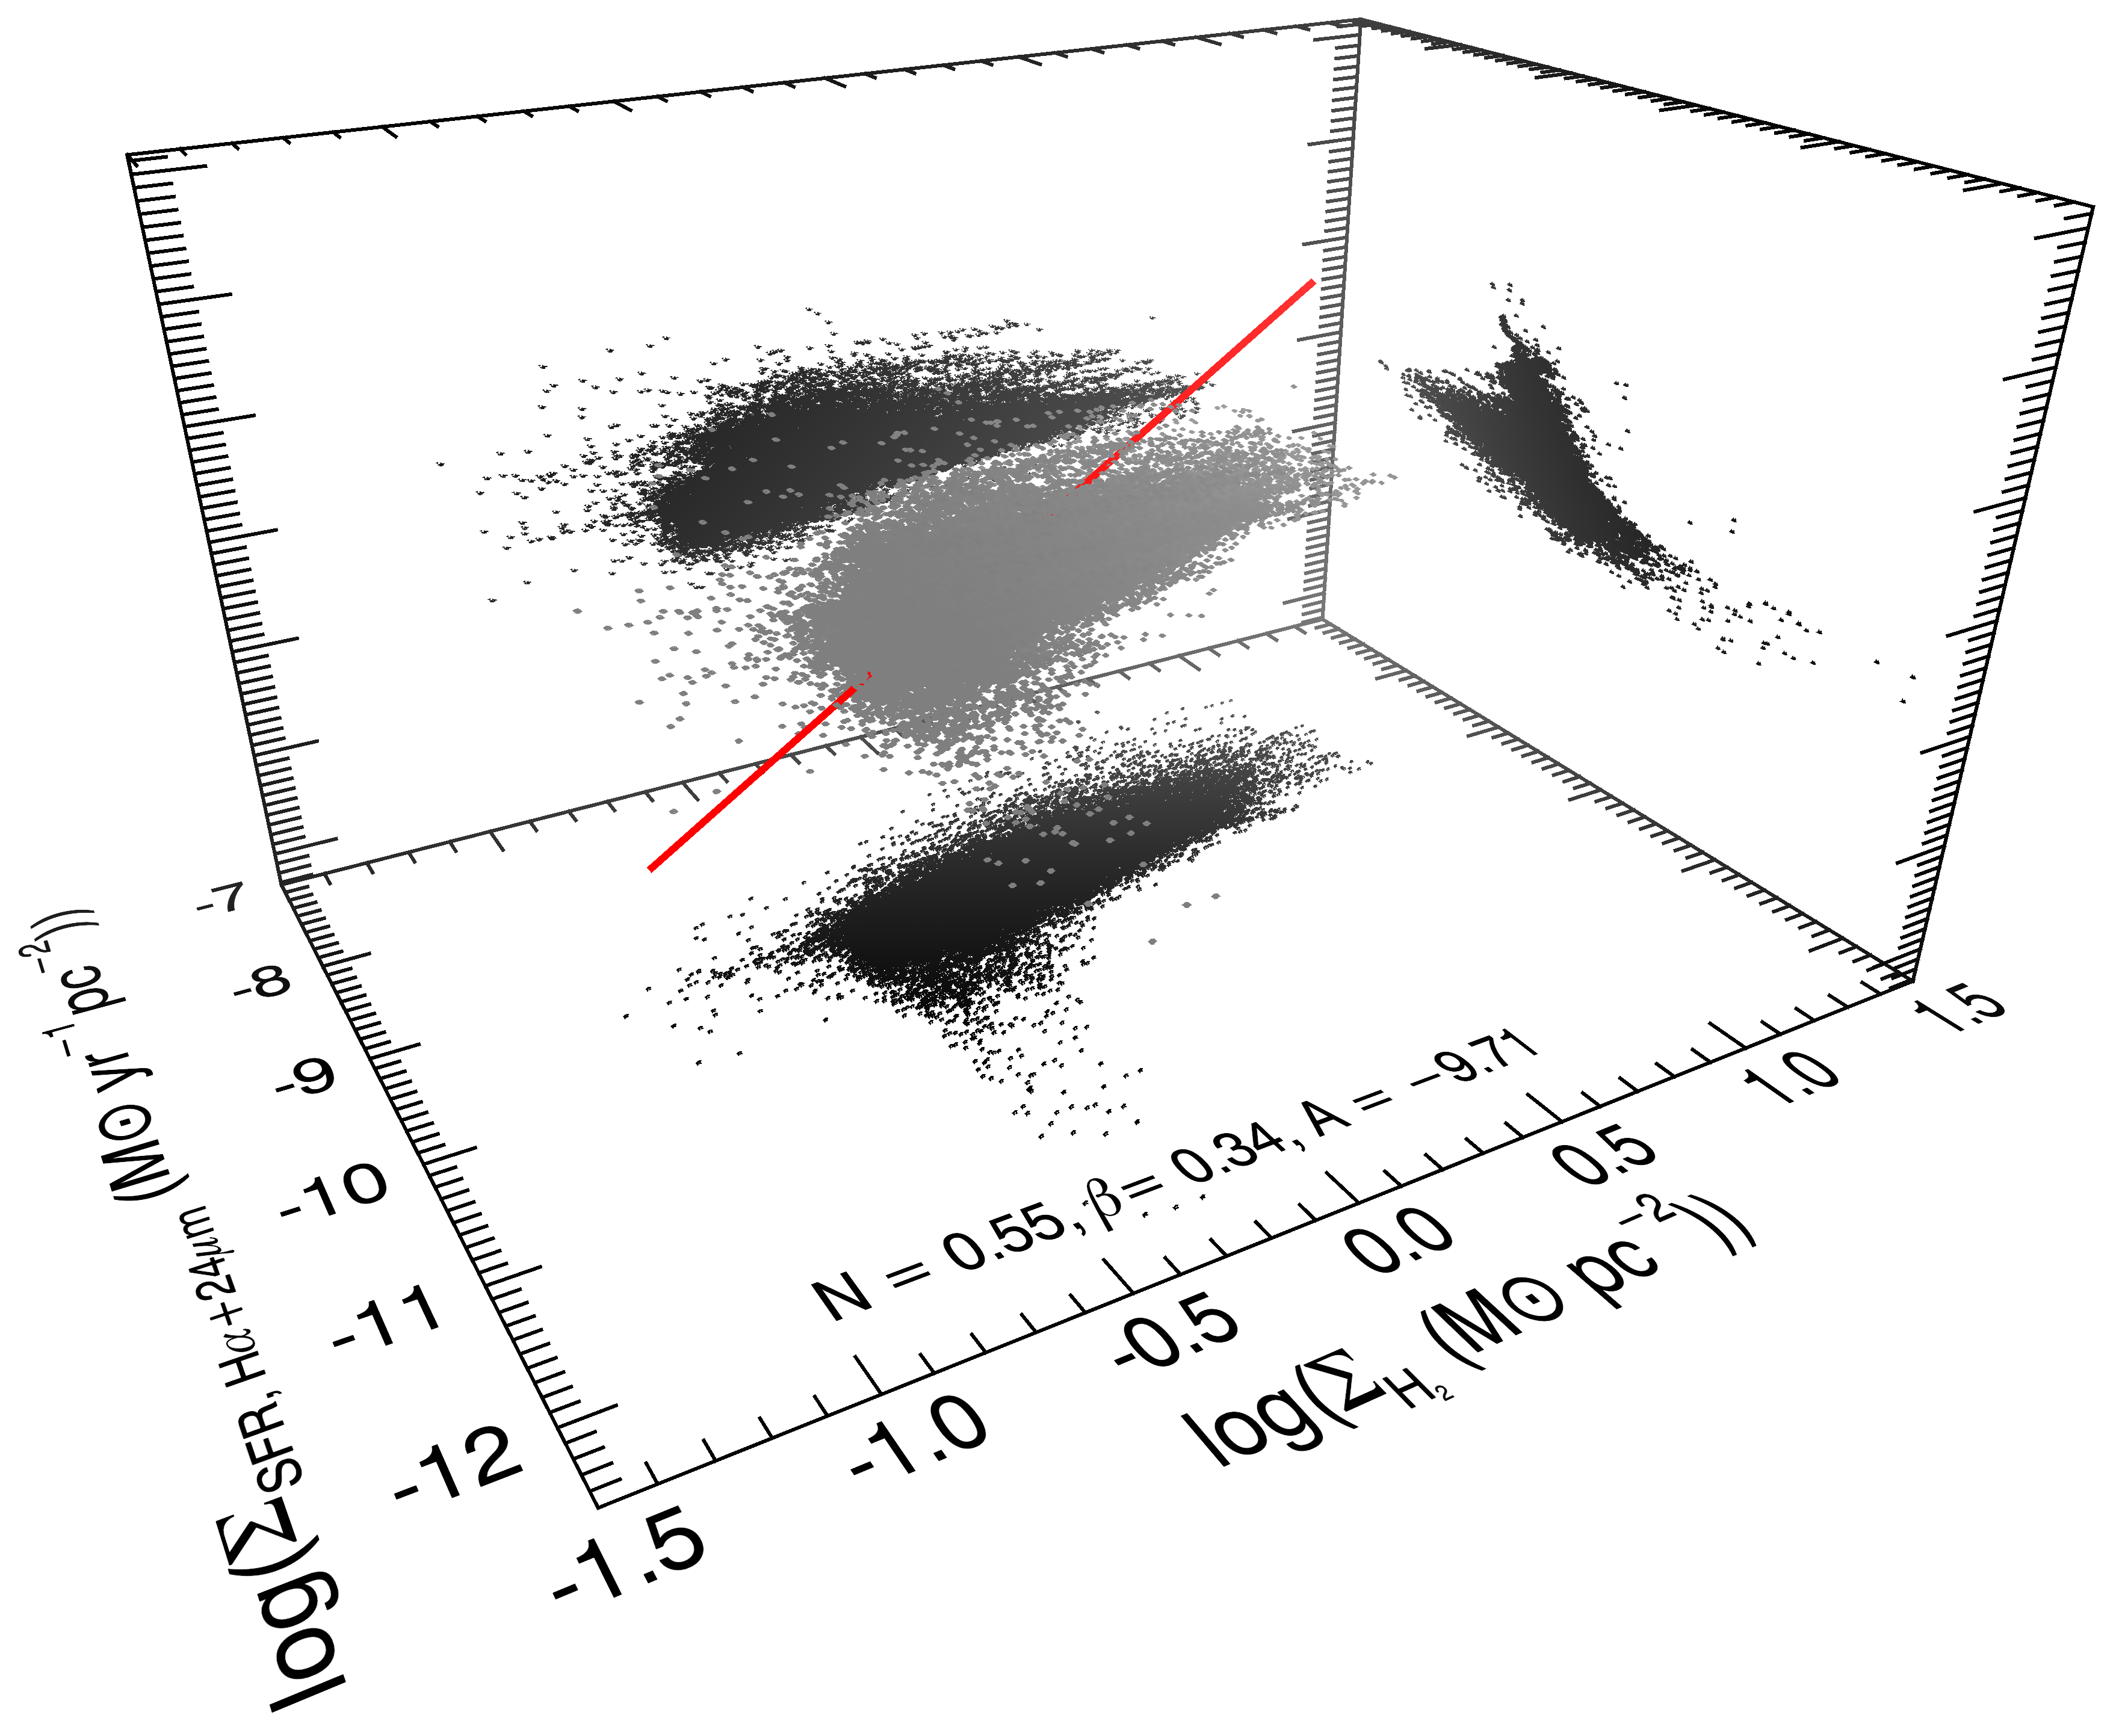
\includegraphics[width=\textwidth]{../image_paper1/es_tot_halpha_vs_h22_f.png}
        \captionsetup{font=tiny}
        \caption{Surface density of SFR(H$\alpha$+24~$\mu$m) vs surface density of H$_2$ and surface density of stellar mass ($z$-axis)}
        \label{fig:es,all,halpha,h2}
    \end{subfigure}
     \hfill
      \begin{subfigure}[b]{0.5\textwidth}
        \centering
        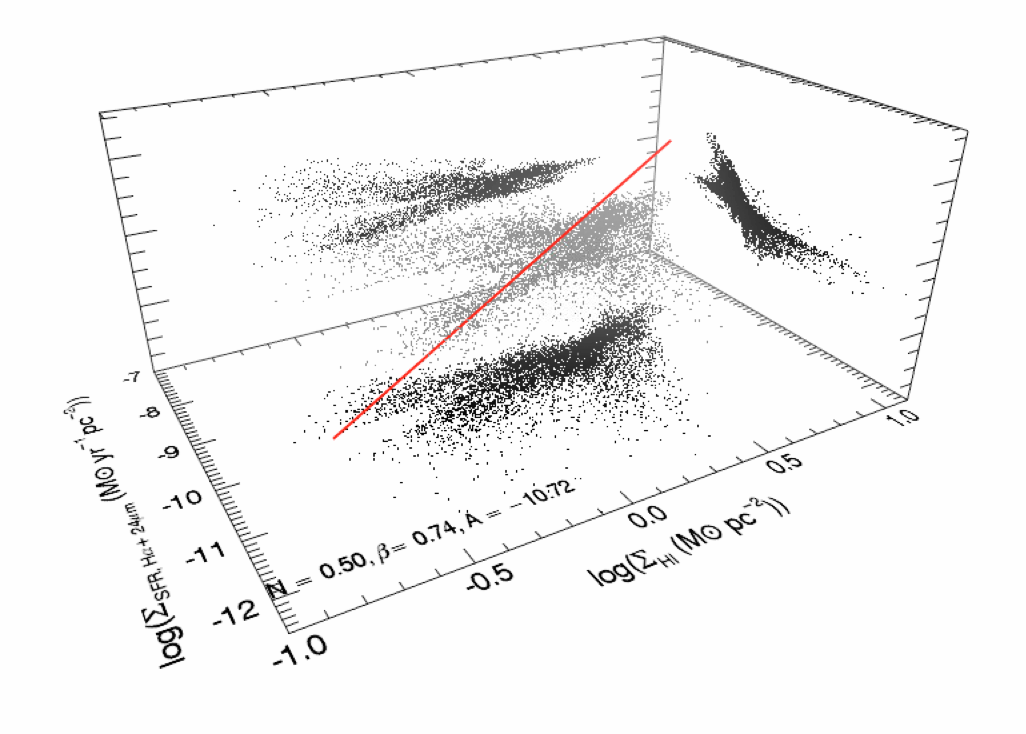
\includegraphics[width=\textwidth]{../image_paper1/es_tot_halpha_vs_hi2.png}
        \captionsetup{font=tiny}
        \caption{Surface density of SFR(H$\alpha$+24~$\mu$m) vs surface density of \hi\ and surface density of stellar mass ($z$-axis)}
        \label{fig:es,all,halpha,hi}
    \end{subfigure}
    \hfill
    \begin{subfigure}[b]{0.5\textwidth}
        \centering
        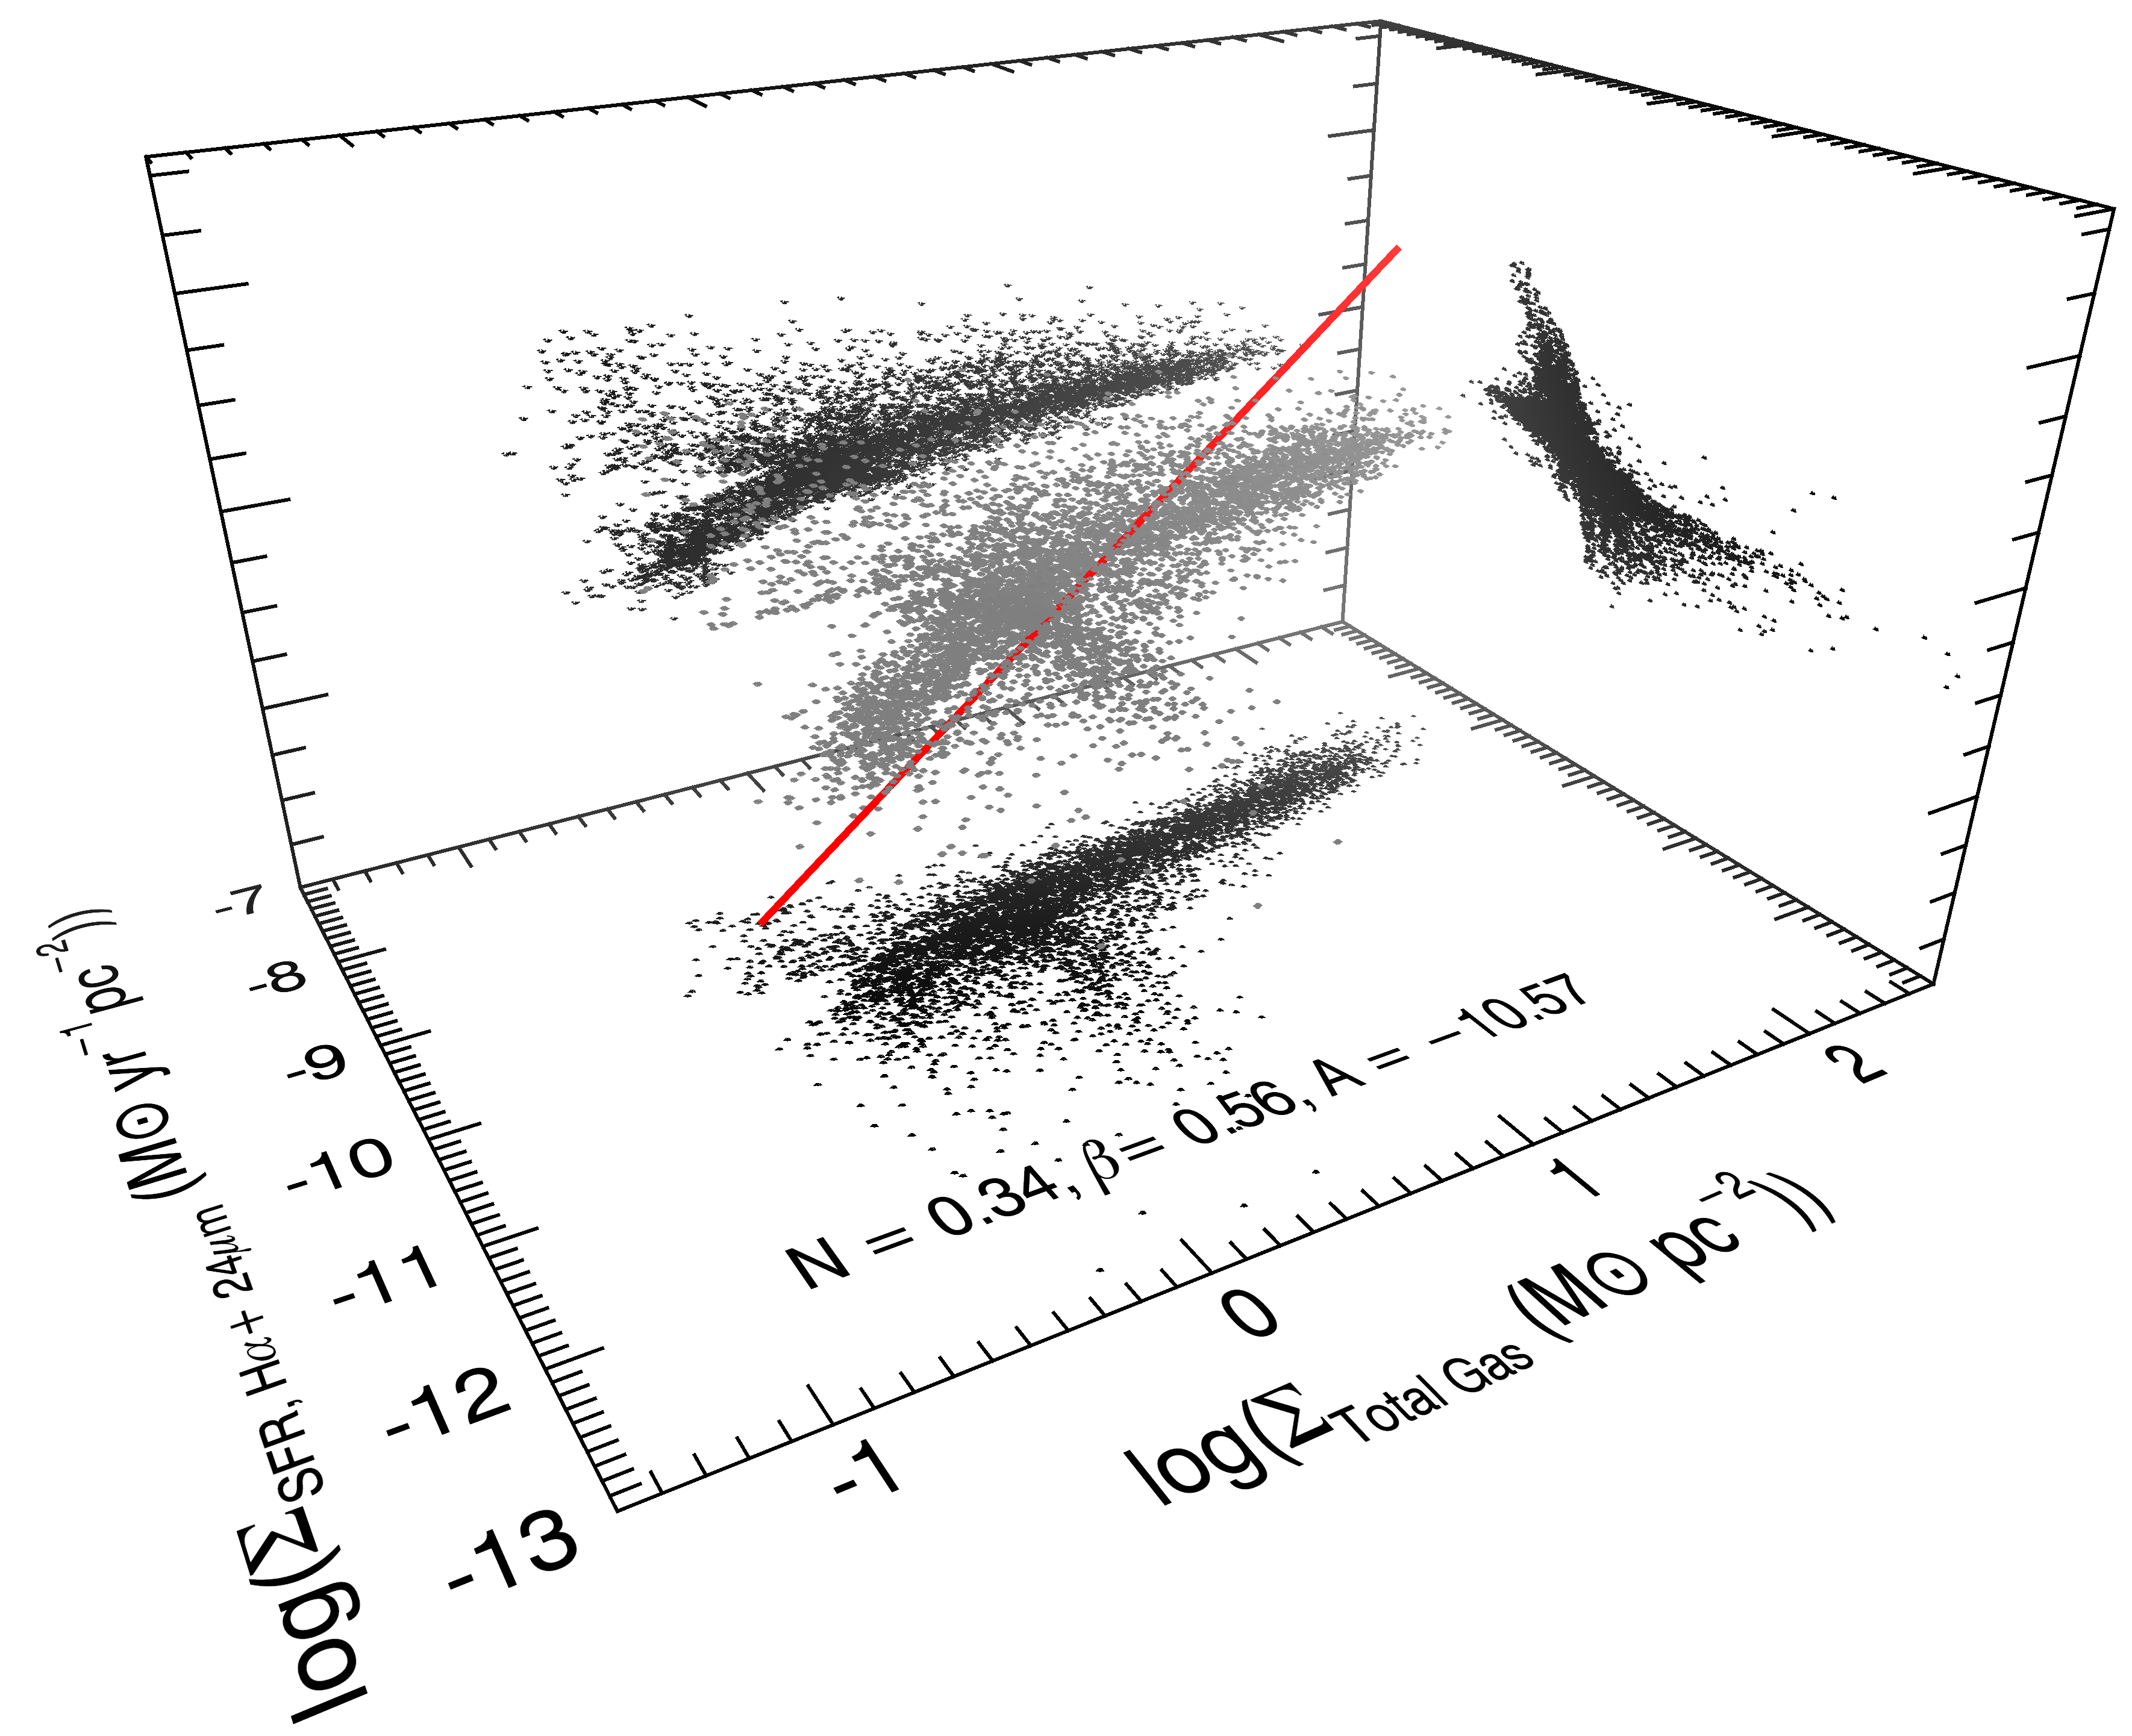
\includegraphics[width=\textwidth]{../image_paper1/es_tot_halpha_vs_tot2_f.png}
        \captionsetup{font=tiny}
        \caption{Surface density of SFR(H$\alpha$+24~$\mu$m) vs. surface density of total gas and surface density of stellar mass ($z$-axis)}
        \label{fig:es,all,halpha,tot}
    \end{subfigure}
    \caption{Same as Fig.~\ref{fig:es,fir}, but in this figure we used H$\alpha$ + 24~$\mu$m as a tracer of the SFR.}
\end{figure}

